% Chapter Template

\chapter{Proposal} % Main chapter title

\label{Proposal} % Change X to a consecutive number; for referencing this chapter elsewhere, use \ref{ChapterX}
%----------------------------------------------------------------------------------------

% Define some commands to keep the formatting separated from the content 
\newcommand{\keyword}[1]{\textbf{\#1}}
\newcommand{\tabhead}[1]{\textbf{\#1}}
\newcommand{\code}[1]{\texttt{\#1}}
\newcommand{\file}[1]{\texttt{\bfseries\#1}}
\newcommand{\option}[1]{\texttt{\itshape\#1}}

%----------------------------------------------------------------------------------------
%	SECTION 1
%----------------------------------------------------------------------------------------

\section{Introduction}

With the projection of rising frequency and intensity of droughts throughout vast parts of the African continent, measures for prediction, monitoring and evidence based anticipatory actions and management become ever more important \autocite{abdulkadirAssessmentDroughtRecurrence2017,adelekanAfricaClimateChange2022,vereintenationenSpecialReportDrought2021}.

In order to meet this challenge, the Red Cross Red Crescent Movement together with the Red Cross Red Crescent Climate Center started the Forecast-based Financing (FbF) programme in 2007 to facilitate Anticipatory Actions instead of post-disaster reactions. Together with their local partners, the International Federation of Red Cross Red Crescent Societies (IFRC) is working on establishing so called Early Action Protocols (EAPs) to ensure better organization and coordination of Anticipatory Actions in the face of an incoming hazard. These actions are based on a predefined interplay of forecast, trigger and financing mechanisms to ensure rapid, scientific based responses.

Somaliland, being no exception to the above mentioned climatic trend, is characterized by droughts with far reaching impacts on ecological, economic, and social aspects. Defined by a semi-arid, four-season climate with two extensive dry seasons and an economic backbone of pastoralism and rain-fed agriculture, water accessibility is of key importance in Somaliland \autocite{abdulkadirAssessmentDroughtRecurrence2017,petrucciLandscapeLandformsNorthern2022,republicofsomalilandSomalilandCountryProfile2021}.
In addition, the final report of the FbF feasibility study identifies five other hazards besides droughts, namely flood, cyclone, disease, locusts and conflict. Of all these hazards, drought was ranked as the greatest threat due to its increasing frequency, severity and wide-ranging consequences.\newline

Existing drought forecasts and trigger indicators are mostly based on physical indicators and cover especially macro- and international levels, e.g. EDDI, SPI, SPEI \todo{look them up + which forecast is defined by the SRCS?}. Fine grained up-to-date forecasts which not only include physical but also social circumstances and knowledge on local levels are often scarce or even non-existent \todo[fancyline]{sources}. "However, assessments focused only on physical variables and processes fail to capture why drought matters [...]."\autocite[3]{lackstromBackyardHydroclimatologyCitizen2022}, how it impacts communities and which mitigation strategies are locally taken \todo{source?}.\newline

Besides the further development of more fine grained technical solutions the integration of local knowledge is another way forward. Engaging local people and communities and giving them an active voice in defining and co-producing anticipatory actions and knowledge can be of multiple benefit to communities and enrich the data generated \autocite{somaliredcrescentsocietyFeasibilityStudyPotential2022, njambi-szlapkaIntegratingCommunityVoices}\todo{source}. On the one hand, citizens can help to fill data gaps of categorized measurements such as simple assessments of dry-to-wet conditions which correspond to the above mentioned technical drought indicators \autocite{lackstromBackyardHydroclimatologyCitizen2022}. On the other hand, citizens can contribute their local knowledge which can potentially draw on years of experience, encompass a wide range of aspects and give them a feeling of co-owning which in itself can already bring many advantages \autocite{njambi-szlapkaIntegratingCommunityVoices}\todo{source}. The IFRC states, that the "community engagement and accountability (CEA) is essential […] to build acceptance and trust” \autocite{ifrcCommunityEngagementAccountability}(IFRC n.d.) for effective and sustainable outcomes. 
Nonetheless, direct contributions and communication from and with volunteers or community members remain a challenge in the joint management of hazards and risks. The tasks are numerous and need to take into consideration different aspects, ranging from cultural differences to different background knowledge and technical capabilities and capacities.

Qualitative interviews can capture a wide range of local contribution, knowledge and information but are very labour intensive, often limited in time and hence not feasible on larger scale for monitoring purposes. Providing a technical solution that enables mutual contact between communities and the Somalia Red Crescent Society (SRCS) in a simple and accessible way would make it possible to collect this most helpful information. By ensuring that sovereignty over the collected data rests with the community, the decision-making power and benefits remain with those concerned. Therefore, in the development and application of an Early Action Protocol (EAP) in the context of Forecast based Action (FbA) in Somalia, the technical aspect in particular holds great potential to benefit numerous communities over the long term.

While there is a comparatively good basis with regard to the general availability of data on social, economic and natural information and conditions, as well as their spatial and qualitative characteristics, the timeliness of this information varies greatly. Especially in the context of Anticipatory Action, time is of the essence and a swift action based on up-to-date data is crucial. Gathering and incorporating local knowledge through manual surveys by a central organisation can be of great value, as shown above, but is time-consuming and slow.

The benefits of overcoming the high labour costs and the temporal handicap by providing a simple and accessible tool for the SRCS’s large network of volunteers can already be seen in other comparable contexts using the Community Based Surveillance (CBS) programme, its successor NYSS, the Ushahidi platform or tools like Social.Water, ITIKI and CoCoRaHS \autocite{fienenSocialWaterCrowdsourcing2012a} \todo{sources}. The CBS is a pioneering technical approach to disease outbreak surveillance in Somalia and was developed as part of the SRCS Health Strategy 2019-2023. In this process, “volunteers report health risks through their respective locations and send to the SRCS data platform […]” \autocite[57]{somaliredcrescentsocietyFeasibilityStudyPotential2022} through coded SMS. So far, 315 volunteers from 115 villages have specifically been trained. In at least two cases, an outbreak could be contained thanks to early detection (SRCS 2021, 2022). On top of this already proven application, further functions could be added as needed.\newline
Social.Water, ITIKI and CoCoRaHS are environmental data collection and drought monitoring implementations. These approaches are based on Crowdsensing approaches and partly employ more sophisticated technical solutions via internet connections, wireless sensor networks or photographs and have been implemented and tested in recent studies or ongoing monitoring programmes. While suggesting that the method of Crowdsensing for data collection and monitoring is fit for purpose, these approaches are not feasible to this context due to internet connection and technical equipment requirements, lack of categorization or their focus on just environmental data acquisition without taking sufficient account of the impact on the community impact and social realities.

The aim of this study is therefore to incorporate local knowledge on the availability of water sources into the monitoring of drought impacts in an effort to support triggering and Anticipatory Actions under the Early Action Protocol. For this purpose, already proven methods are combined. First, semi-structured (expert-) interviews will be conducted to generate in-depth local knowledge. Based on these findings on local (pre-)conditions, needs and limitations, a monitoring tool based on a volunteersensing approach will then be conceptualized and subsequently discussed with local decision-makers. A prototype development based on the Social.Water tool is a further possibility. In addition, the question of the equality of local to scientific knowledge will be raised and further influences of such a contribution on social conditions will be investigated \todo{too much?}.

This work is thus based on the question \textit{"In what way can a collaborative Volunteer Sensing Approach be conceptualized to facilitate community water source monitoring in Somaliland in order to enhance early drought triggers and following Anticipatory Actions?"} and explores following hypotheses:\newline
1. Local knowledge can enhance early drought impact triggers in the context of Anticipatory Actions in Somaliland.\newline
2. Water source availability, accessibility and quality are feasible ecological and social indicators for monitoring early drought impacts and guide Anticipatory Actions in Somaliland.\newline
3. The combination of qualitative interviews and Volunteered Crowdsensing is a promising approach to qualitatively and quantitatively monitor early drought impacts on communities in Somaliland.\newline

\subsection{Timeline}
\begin{figure}[h]
    \centering
    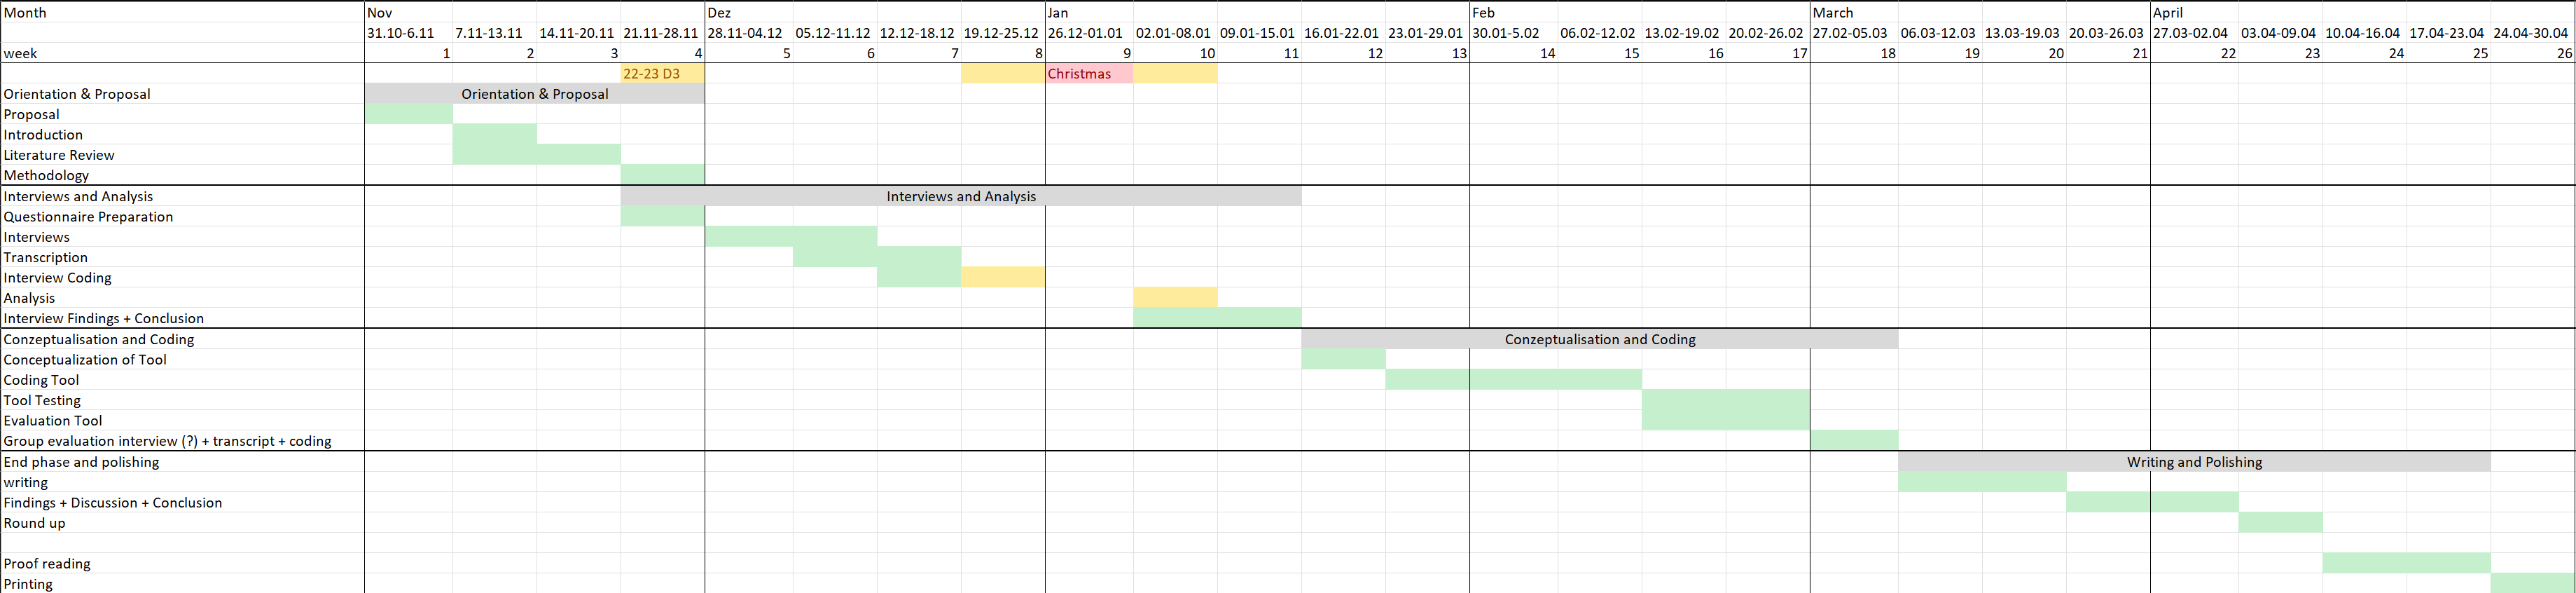
\includegraphics{Figures/SottmannBosse_timeline.png}
    \caption[Timeline Master Thesis]{Timeline Master Thesis}
    \label{fig:timeline}
    \end{figure}
    
\subsection{Outline}:
Declaration of Authorship
Abstract
Acknowledgements
Contents
List of Figures
List of Tables
List of Abbreviations

1.  Chapter: Introduction (eher ausbauen oder eher in den Literature Review Part?)
    1.1. Motivation
    1.2. General introduction and overview
    1.3. Structure
2.  Theoretical Introduction
    2.1. Case Study Area (Somalia, Somaliland, etc.)
    2.2. Project FbF and EAP (project, goal, requirements, work, context)
    2.3. Water source Monitoring – State of the Art (satellite imagery, upside, downside)
    	2.3.1. Types of Water sources
    	2.3.2. Types of transport (?)
    	2.3.3 The Case of Genders
	2.4. VGI and Crowdsensing (Ups and Downs + benefit)
    2.5. Tool and Programme introduction (overview tools, downside of tools in place, possible solution)
    2.5.1. Requirements ( based on interviews)
    2.5.2. Communication tools
    2.5.3. Data collection
    2.5.4. Data cleaning
    2.5.5. Data processing
    2.5.6. Data analysis
    2.5.7. Data Display/depiction/representation
3.  Methodology (empirical research)
    3.1. Literature/existing tools review
    3.2. Half-structured interviews
    3.2.1. With whom, how, when,
    3.2.2. About what (creation of questionnaire)
    3.2.3. Why did NYSS and other programmes not succeed?
    3.2.4. Coding + qualitative and quantitative (?) analysis
    3.2.5. Evaluation and Conclusion
    3.2.6.
    3.3. Conceptualization of a solution
    3.3.1. Synthesis Outcome Interviews + Review other Tools
    3.3.2. Structure of functioning
    3.3.3. Restructuring existing 2.7 Python Tool and Extending it
    3.3.4. Testing / Evaluation (if possible?)
4.  Results
    4.1. Literature
    4.2. Interviews
    4.3. Conceptualization
    4.4. Actual Tool
    4.5. Evaluation (?)
5.  Discussion
    5.1. Discussion methodology
    5.2. Discussion Results
    5.3. Discussion Evaluation
    5.4. Limitations
6.  Conclusion and Future outlook
7.  Eidesstattliche Erklärung
8.  References
9.  Attachements

\todototoc
\listoftodos